Im Folgenden soll auf den verwendeten experimentellen Aufbau eingegangen werden. 
Dafür wird dieser zuerst anhand einer Skizze erklärt. 
Anschließend wird die bereits entwickelte Theorie auf den Aufbau bezogen und aufgezeigt, welche Abweichungen sich von der idealisierten Herangehensweise im vorangegangenen Abschnitt ergeben. 
In diesem Zuge wird abschließend die Erwartung an die Messgröße $\tau_c$ berechnet, auf welche sich in späteren Abschnitten bezogen werden soll. \\

Am Einfachsten lässt sich der Versuchsaufbau anhand einer vereinfachten Skizze nachvollziehen. Diese ist daher in \autoref{fig:Versuchsaufbau} dargestellt. 
\begin{figure}[h]
    \centering
    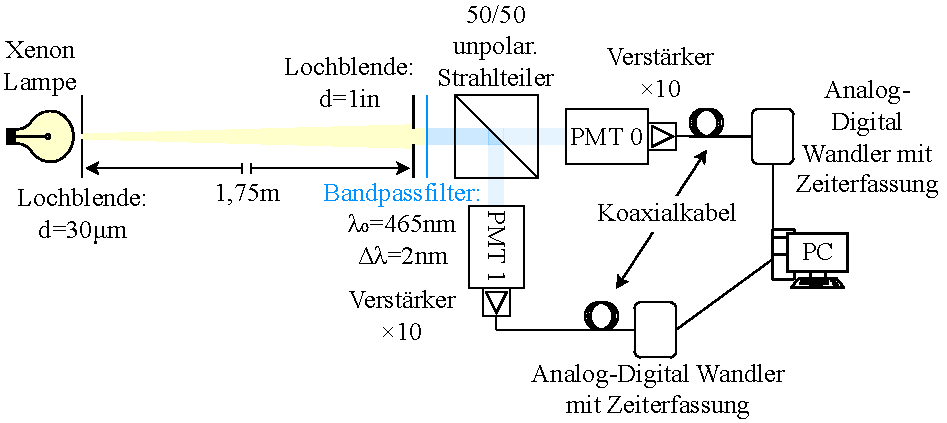
\includegraphics[width=0.9\linewidth]{images/Aufbau/Aufbau.pdf}
    \caption{Abgebildet ist eine vereinfachte Skizze des verwendeten Aufbaus, welche die konzeptuell wichtigsten Bauteile darstellt.}
    \label{fig:Versuchsaufbau}
\end{figure}
\todo{Farbe vom Bandpass passt nicht}
Als Lichtquelle wird eine Xenon Lampe (\todo{lampentyp}...) gewählt. 
Als Gasentladungslampe emittiert diese nach \autoref{ssec:Intensitäteninterferometrie} chaotisches Licht, welches Bunching aufweist. 
Da nach dem van Cittert-Zernike-Theorem der Winkeldurchmesser der Lichtquelle invers proportional zur Breite von $g^{(2)}(\bm{\rho})$ ist, ist weiterhin darauf zu achten, die Ausdehnung der Lichtquelle einzuschränken, damit überhaupt korrelierte Photonen am Detektor vorliegen. 
Zu diesem Zweck ist eine kreisförmige Lochblende mit einem Durchmesser von $d=30\,\mathrm{\mu m}$ verbaut. 
Mit der Distanz $x=1,75\,\mathrm{m}$ zwischen Lichtquelle und dem restlichen Aufbau ergibt sich so ein Winkeldurchmesser von $\Delta \theta \approx \frac{d}{x} = 3,53\,\mathrm{asec}$. 
Es sei darauf hingewiesen, dass die größten Winkeldurchmesser von Sternen im Bereich von tausendstel Bogensekunden liegen \cite{hanburybrownAngularDiameters321974}, also etwa drei Größenordnungen kleiner sind, als der hier geschaffene \glqq künstliche Stern\grqq. \\
Um dem eintretenden Lichtstrahl eine definierte Breite zu geben, wird dieser zusätzlich durch eine Lochblende mit einem Durchmesser von einem Zoll geleitet. 
\todo{warum?}
Wie in \autoref{ssec:Michelson-Sterninterferometer} beschrieben, ist für eine Messung der räumlichen Kohärenz auch eine nicht verschwindende Kohärenzzeit relevant. 
Da diese indirekt proportional zur spektralen Breite der Quelle ist, wird an dieser Stelle ein enger Bandpassfilter (Alluxa 465-2 \cite{4652OD4Ultra}) mit einer annähernd rechteckförmigen Transmissivität verbaut. 
Dieser hat nach Herstellerangaben eine zentrale Wellenlänge von $\lambda_0 = 465\,\mathrm{nm}$ und eine Halbwertsbreite von  $\Delta\lambda = 2\,\mathrm{nm}$. 
Anschließend wird der Strahl durch einen nicht polarisierenden 50/50 Strahlteilerwürfel (Thorlabs BS031 \cite{ThorlabsBS03150}) aufgeteilt und zum Nachweis der Photonen auf zwei Photomultiplier (PMTs) gelenkt. 
Um bei hohen Photonenraten weiterhin eine lineare Verstärkung durch die PMTs zu erhalten, werden die letzten vier Dynoden mit einer Stabilisationsspannung betrieben \cite{zmijaOpticalIntensityInterferometry2021}. 
Als Spannungsquelle für die Hochspannung und die Stabilisationsspannung wird eine durch den Computer steuerbare Spannungsquelle (CAEN DT5533E \cite{DT5533E}) genutzt. 
Direkt am Ausgang der Photomultiplier (\todo{pmttyp}...) werden die Pulse mit einem Verstärker (FAST ComTec TA1000B-10 \cite{TA1000BTimingAmplifier}) um den Faktor 10 verstärkt. 
Die Verstärkung direkt an den PMTs hat den Vorteil, dass Störsignale nicht vor der Verstärkung einkoppeln können, was das Signal-Rausch-Verhältnis verbessert. 
Anschließend werden die Signale durch variable Kombinationen an Kabellänge und -modell zu Analog-Digital-Wandlern (Spectrum M4I.2212-X8 \cite{M4i2212x8Bit}) geleitet, wo diese digitalisiert werden. 
Obwohl jede der Spektrum-Karten vier Digitalisierungskanäle unterstützt, werden zwei verschiedene und räumlich getrennte Karten genutzt, um ein Übersprechen zwischen den Kanälen zu verhindern. 
Aufgrund des von Natur aus geringen Signals werden alle analogen Signale durch geschirmte Koaxialkabel geleitet, um das Einkoppeln von Störsignalen zu erschweren. 
Um zusätzlich das Einkoppeln von störendem Licht des PCs oder sonstiger LEDs der Messgeräte zu erschweren, ist der optische Aufbau zudem durch ein Thorlabs-Röhrensystem fest verbunden, sodass nur Licht entlang der optischen Achse eindringen kann. 
Die zeitliche Synchronisierung der Waveforms zur späteren Korrelation erfolgt durch Verwendung des White Rabbit Systems (vgl. z. B. \cite{lipinskiWhiteRabbitPTP2011}), welches direkt mit den Analog-Digital-Wandlern (ADCs) verbunden ist. 
Abschließend werden die Daten auf RAIDs (Areca ARC-8050T3U-12 \cite{ARC8050T3UThunderboltUSB}) zur späteren Korrelation gespeichert. \\
Da ein Ziel dieser Arbeit ist, zu untersuchen, wie sich verschiedene Kabel auf das Integral des Bunching Peaks auswirken, soll an dieser Stelle explizit auf die verwendeten Koaxialkabel eingegangen werden. 
Die ersten durchgeführten Messungen erfolgen mit 10 und 40\,m langen Kabeln des Typs Airborne 5 \cite{s.r.lAirborne10Coaxial}. 
Dies entspricht den Kabeln, welche in der von der Arbeitsgruppe 2022 durchgeführten Kampagne mit den H.E.S.S.-Teleskopen genutzt wurden \cite{zmijaFirstIntensityInterferometry2023}. 
Anschließend wurden noch Messungen mit Kabeln des Typs LMR400 durchgeführt \cite{LMR400CoaxCable}. 
Diese weisen eine geringere Dämpfung auf als die Airborne 5 Kabel und sind daher interessant, um den Einfluss der Dämpfung auf die gemessene $\tau_c$ zu untersuchen. \\

Aufgrund des speziellen Aufbaus ergeben sich einige Änderungen bezüglich der im vorangegangenen Abschnitt eingeführten Theorie. 
Auf diese soll hier eingegangen werden. 
Wie erwähnt ist der Winkeldurchmesser der Quelle vergleichsweise groß. 
Nach \autoref{eq:erste nulstelle von g2(rho) für lochblende} wird für die Distanz zur ersten Nullstelle der $g^{(2)}$-Funktion lediglich $\rho_0\approx3,3\,\mathrm{cm}$ erwartet. 
Das heißt, dass am Beobachtungsort lediglich in einem Kreis mit Radius $\rho_0$ korrelierte Photonen auftreten. 
Aufgrund der physischen Größe der PMTs ist es daher nicht möglich, $g^{(2)}(\rho)$ für verschiedene $\rho$ zu messen. 
Stattdessen wird ein Mittelwert von $g^{(2)}$ in einem Intervall von $\rho\in[0,1]$ Zoll gemessen. 
Dieses Intervall entspricht den Abständen, die korrelierte Photonen durch die Lochblende am Eingang des Strahlteilers haben können. 
Es wird also erwartet, einen erniedrigten Wert für $g^{(2)}(\rho)$ und damit $\tau_c$ zu messen. 
Dies ist in \autoref{fig:räumliche koh simulation} verdeutlicht. 
\begin{figure}[h]
    \centering
    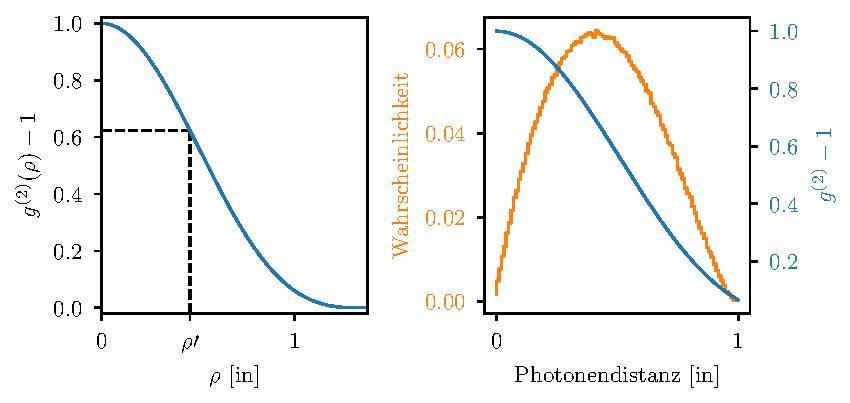
\includegraphics{images/Aufbau/g2(rho).pdf}
    \caption{Dargestellt ist links die $g^{(2)}$-Funktion, abhängig von der Separation $\rho$. Rechts ist das Ergebnis der Simulation abgebildet. In Blau ist $g^{(2)}$ für jeden Photonenabstand dargestellt (dies entspricht der Kurve im linken Graphen), während in Orange die simulierte Wahrscheinlichkeitsverteilung, ein Photonenpaar bei gegebenem Abstand anzutreffen, aufgetragen ist. Durch Multiplikation der beiden Kurven erhält man den Faktor, wie viel räumliche Kohärenz im Vergleich zum Maximum noch vorhanden ist. Dieser beträgt $k_s=0,62$. Links ist zudem eingezeichnet, welchem Abstand $\rho\prime$ diese Kohärenz entsprechen würde. }
    \label{fig:räumliche koh simulation}
\end{figure}
Um herauszufinden, um welchen Faktor die gemessene Amplitude von der theoretischen maximalen Amplitude abweicht, wird eine Simulation durchgeführt, die sowohl den Wert von $g^{(2)}$ für jeden Photonenabstand als auch die Wahrscheinlichkeit für diesen berücksichtigt. 
Der Faktor, um welchen $g^{(2)}$ im Vergleich zu $g^{(2)}(0)$ verringert ist, beträgt bei gegebenem Aufbau $k_s=0,62$. 
\todo{Wie zitiere ich diese Simulationen?}
Über den theoretischen Verlauf der Korrelationsfunktion lässt sich durch $k_s$ auf einen effektiven Teleskopabstand $\rho\prime$ schließen, bei dem ein dünner Strahl denselben Verlust an räumlicher Kohärenz aufweist. 
Dies ist auch in \autoref{fig:räumliche koh simulation} veranschaulicht. \\

Aus voriger Überlegung ist nun bekannt $\tau_c^{meas} = k_s\cdot\tau_c^{th}$. 
Um $\tau_c^{th}$ zu bestimmen, wird eine weitere Simulation verwendet. 
Diese berechnet aus dem vom Hersteller gegebenen Transmissionspektrum des Filters über das Wiener-Khintchine-Theorem, d. h. eine Fouriertransformation, die erwartete $g^{(1)}$-Funktion, welche anschließend über die Siegert-Relation in $g^{(2)}(\tau, \rho=0)$ umgerechnet wird. 
Daraus folgt dann für den vorliegenden Fall $\tau_c^{th} = \int g^{(2)}(\tau, \rho=0) -1 = 0,152\,\mathrm{ps}$. 
Abschließend ergibt sich also für die erwartete Kohärenzzeit bei verwendetem Aufbau:
\begin{equation}
    \tau_c^{meas} = 0,152\,\mathrm{ps}\cdot 0,62 = 94\,\mathrm{fs}
    \label{eq:tau_c_th}
\end{equation}


